\documentclass{article}
\usepackage{fullpage}
\usepackage{amsmath}
\usepackage{graphicx}
\renewcommand{\familydefault}{\sfdefault}

\begin{document}
\title{H\"uckel theory applied to molecular motors}
\author{Jurn Heinen}
\maketitle

In 2016, the Chemistry Nobel Prize was awarded to Fraser Stoddart, Jean-Pierre Sauvage and Ben Feringa "for the design and synthesis of molecular machines”.\cite{nobelprizechemistry2016} A special type of these molecular machines is the molecular motor. A molecular motors has light-addressable switches and can isomerize under the influence of UV-light.\cite{Feringa2012} The unidirectional rotation of a motor was first reported in 1999 using UV-radiation and thermal relaxation.\cite{Koumura1999} This lead to the radical idea that these molecular motors can be used potentially as nanorobots used in drug delivery. An example is shown in Figure \ref{fig:mm1} of how molecular motor 1 isomerizes at $\lambda$ = 395 nm.

\begin{figure}[h]
\centering
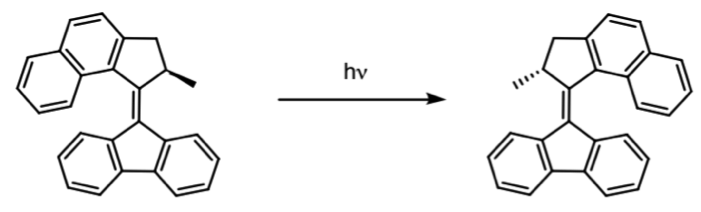
\includegraphics[scale=0.75]{./images/scheme1.png}
\caption{Molecular motor 1 isomerizes using a wavelength of $\lambda$ = 395 nm.}
\label{fig:mm1}
\end{figure} 

However, UV-light can damage biological matter. Therefore, it is crucial that the excitation wavelength needed for isomerization could be reduced to lower wavelengths. A recent experimental study by Feringa et al. showed that extending the aromatic core by substituting the benzene-core by a naphthalene-core, see Scheme \ref{fig:mm2}, can red-shift the excitation wavelength of the molecular motor.\cite{VanLeeuwen2017} 

\begin{figure}[h]
\centering
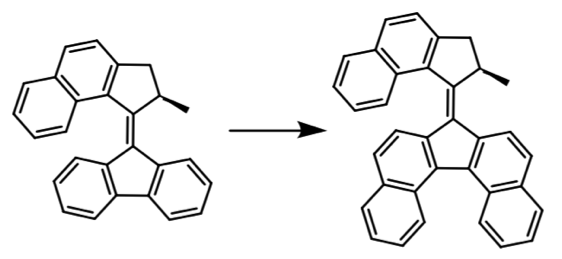
\includegraphics[scale=0.75]{./images/scheme2.png}
\caption{Substitution of the aromatic core of molecular motor 1 by a naphthalene causes a red-shift of the excition wavelength to 491 nm.}
\label{fig:mm2}
\end{figure} 

Using HuLiS, this red-shifting can be predicted by comparing the HOMO-LUMO gaps of both motors. The HOMO-LUMO gap of motor 1 is ELUMO - EHOMO = ($\alpha$ − 0.28$\beta$) - ($\alpha$ + 0.43$\beta$) = -0.71$\beta$. It is expected that the same gap should be calculated for motor 2. Feringa et al. found that the HOMO-1 to LUMO excitation has a significant larger oscillator strength (0.6241) than that of the HOMO to LUMO excitation (0.0105) for molecular motor 2. A higher oscillation strengths implies a large transition probability for excitation.11 Therefore, the excitation energy for motor 2 is calculated from the HOMO-1 LUMO gap and results in ($\alpha$ - 0.21$\beta$) - ($\alpha$ + 0.47$\beta$) = -0.68$\beta$. Since $\beta {<} 0$, the red-shift is indeed predicted. Moreover, visualization of the HOMO, HOMO-1 and LUMO of motors 1 and 2, shown in Figure \ref{fig:hulis_orbitals}, agree surprisingly well with TD-DFT (B3LYP 6-31(d,g)) calculations of Fergina et al.

\begin{figure}[h]
\centering
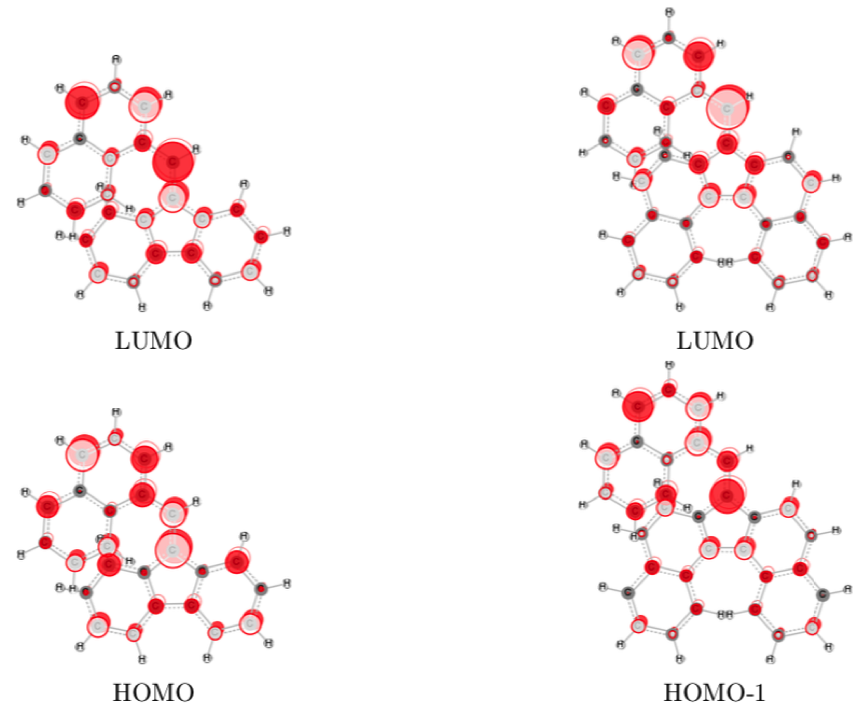
\includegraphics[scale=0.75]{./images/hulis_mm.png}
\caption{Molecular orbitals of motor 1 (left) and motor 2 (right) genereated with HuLiS.}
\label{fig:hulis_orbitals}
\end{figure} 

\bibliographystyle{plain}               
\bibliography{references.bib}    

\end{document}